In general, results from the new system are much smoother than results from the existing system, which include quite a lot of noise. [\textbf{Future: Analyzing signal-to-noise ratio of these results.}] We suspect that this is a consequence of using wide-field illumination, as is done in the existing system, in which molecules outside the region of interest (or otherwise, with some defects) are excited and emit spectra different from that of the region of interest.[\textbf{Needs citation}]

\section{ADT TES-F}

For a drop-cast sample of ADT TES-F on glass, we selected a region of interest which appeared to be a single crystal, with few visually distinguishable defects. The crystal was also selected such that its surface area was larger than the area illuminated by the new system's laser beam. The emission spectra of the region of interest are shown in Figure \ref{fig:pl-adt-tesf}.

[\textbf{Future: Convert wavelength from nm to eV. This seems to be a more common unit in solid state.}]

Both spectra in Figure \ref{fig:pl-adt-tesf} show a clear peak around 630nm, which has been reported in other research. [\textbf{Needs citation. Perhaps Ostroverkohva? 10.1117/12.875375}] The spectra measured by the new system also shows a secondary peak near 600nm, which is not evident in the spectra taken by the existing system.

\begin{figure}[h]
    \centering
    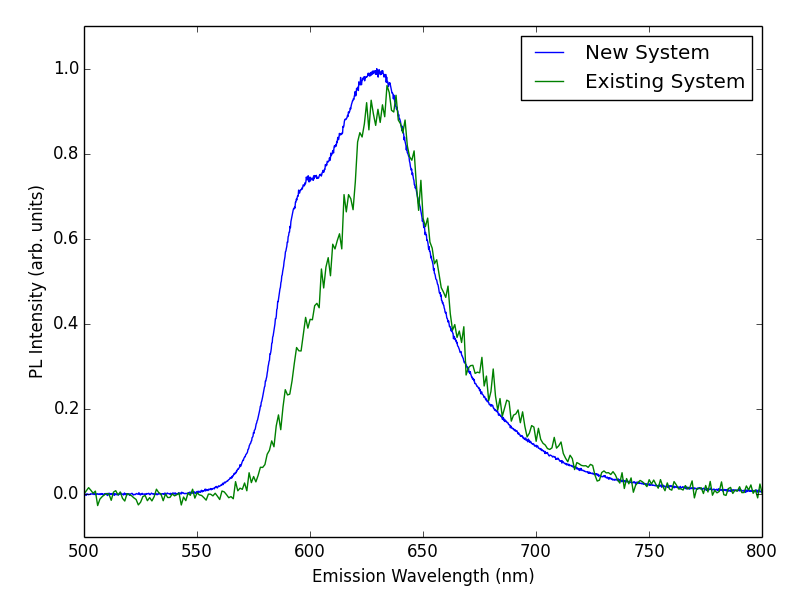
\includegraphics[width=.8\textwidth]{./img/tesf-2.png}%\llap{\raisebox{4cm}{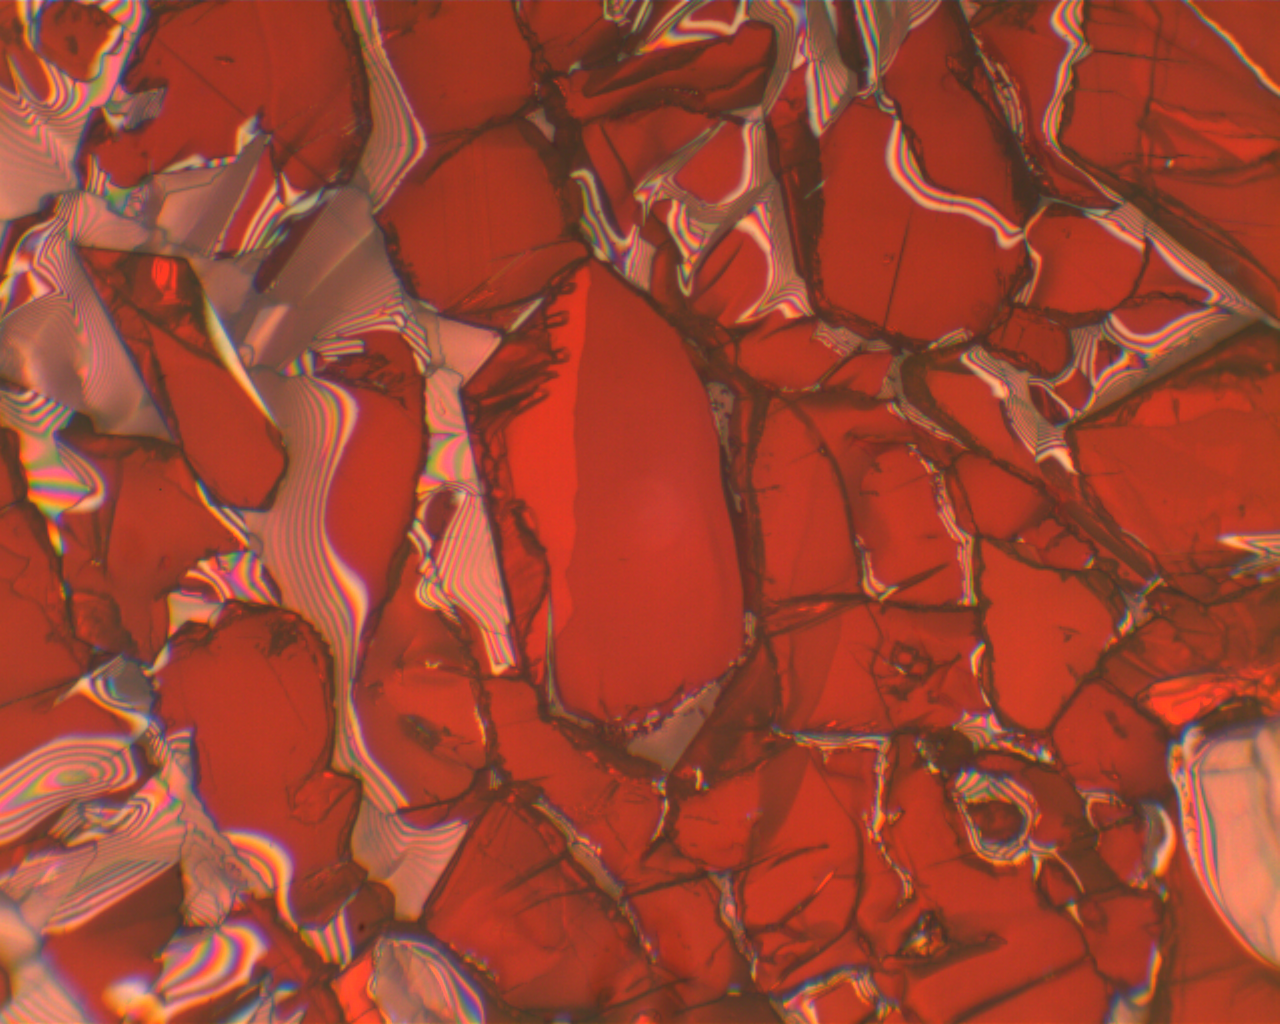
\includegraphics[width=2cm]{img/tesf-white-illum.png}}}
    % 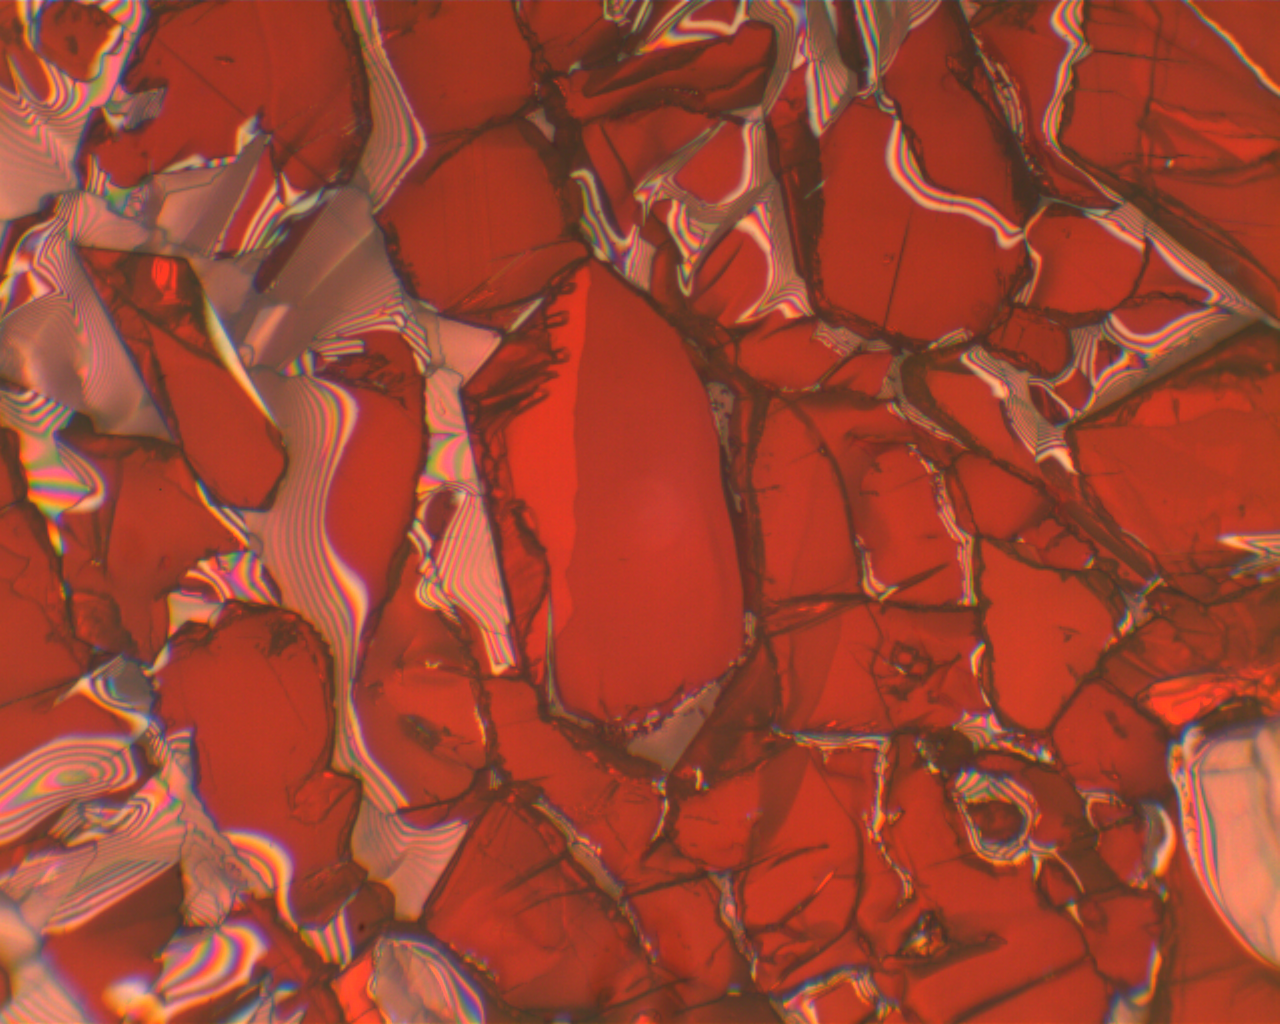
\includegraphics[width=.2\textwidth]{./img/tesf-white-illum.png}
    % 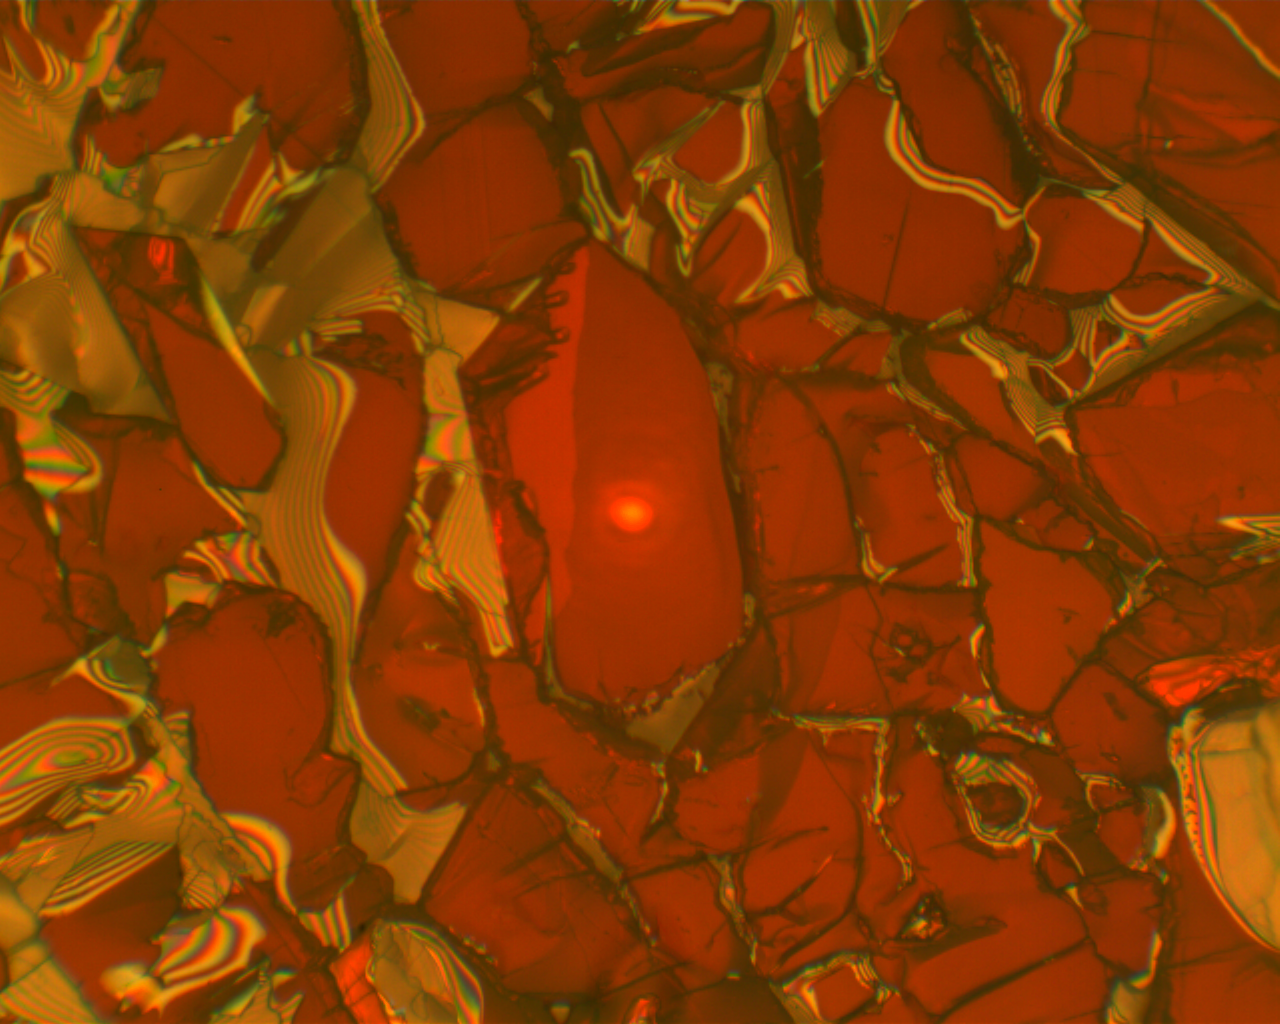
\includegraphics[width=.2\textwidth]{./img/tesf-laser-illum.png}
    \caption{PL emission spectrum of ADT TES-F, excited at 405 nm.
    Wide-field illumination used by the existing system to excite the sample
    yields a noisy spectrum, and does not excite the secondary peak that is 
    shown clearly in the results from the new system. A single crystal, larger than the laser spot, was selected among smaller neighboring crystals for this measurement. %This may be because the
    %wide-field illumination is exciting many adjacent crystals in the sample, 
    %which emit slightly different spectra. The laser illumination in the new 
    %system has the spatial resolution necessary to illuminate single crystals.
    }
    \label{fig:pl-adt-tesf}
\end{figure}

\section{\ce{CdSe} Quantum Dots}

[\textbf{Coming soon.}]

\begin{figure}[h]
    \centering
    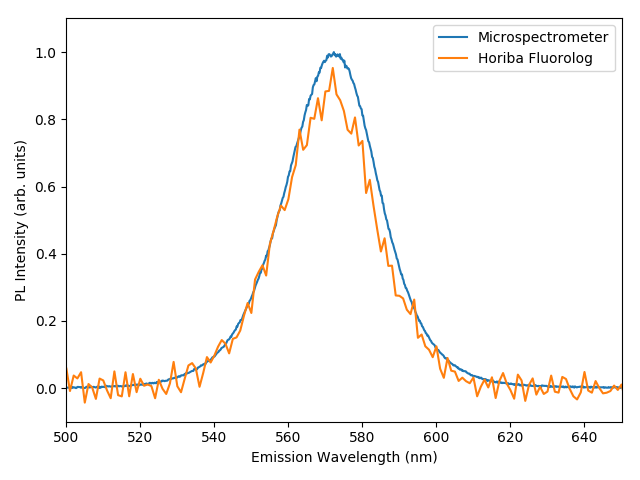
\includegraphics[width=\textwidth]{./img/qd-2.png}
    % 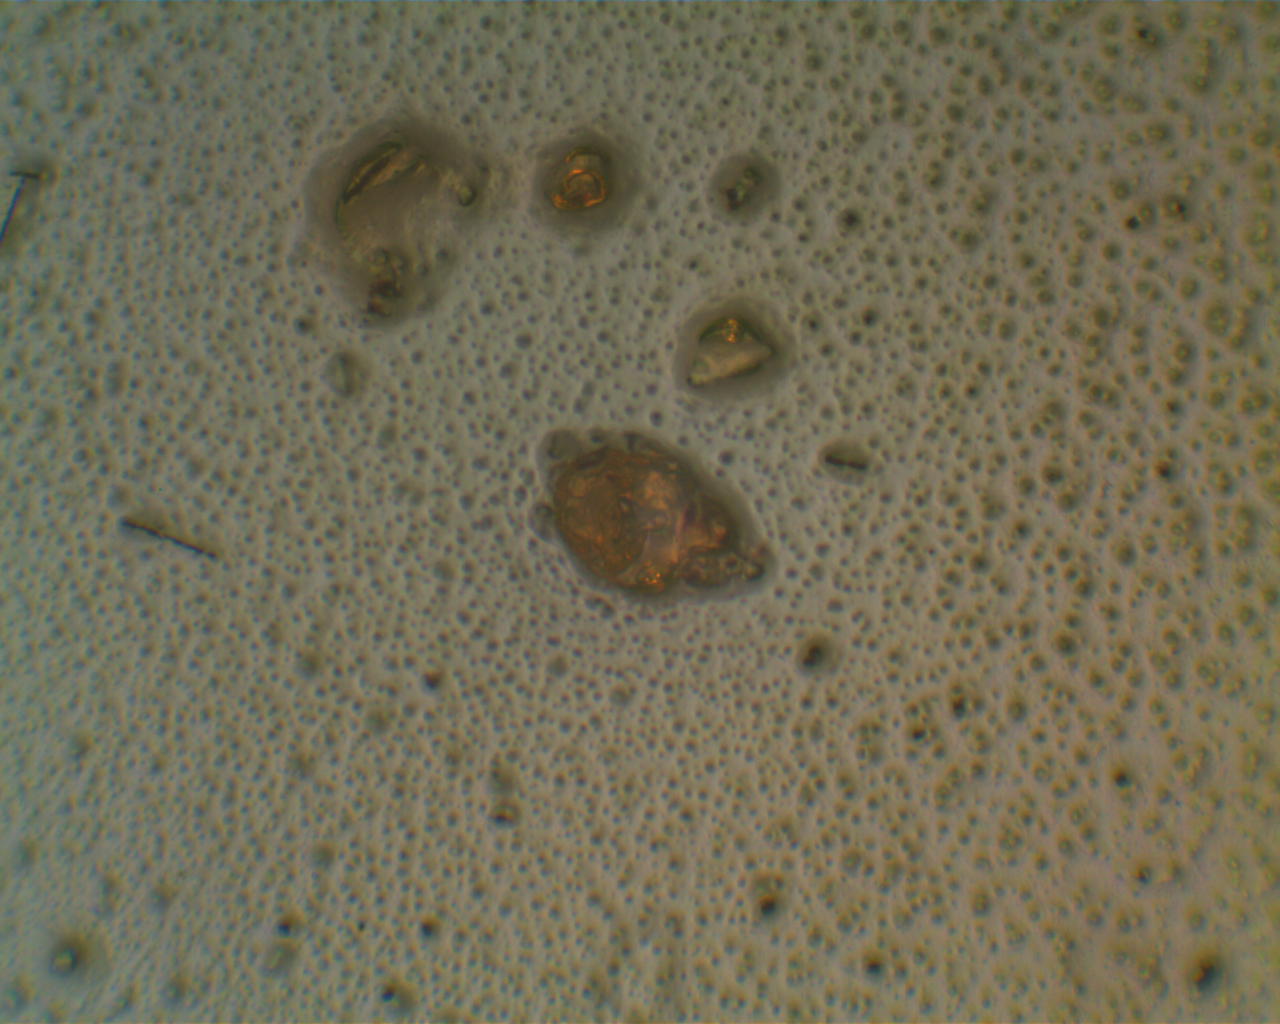
\includegraphics[width=4cm]{./img/qd-white-illum.png}
    % 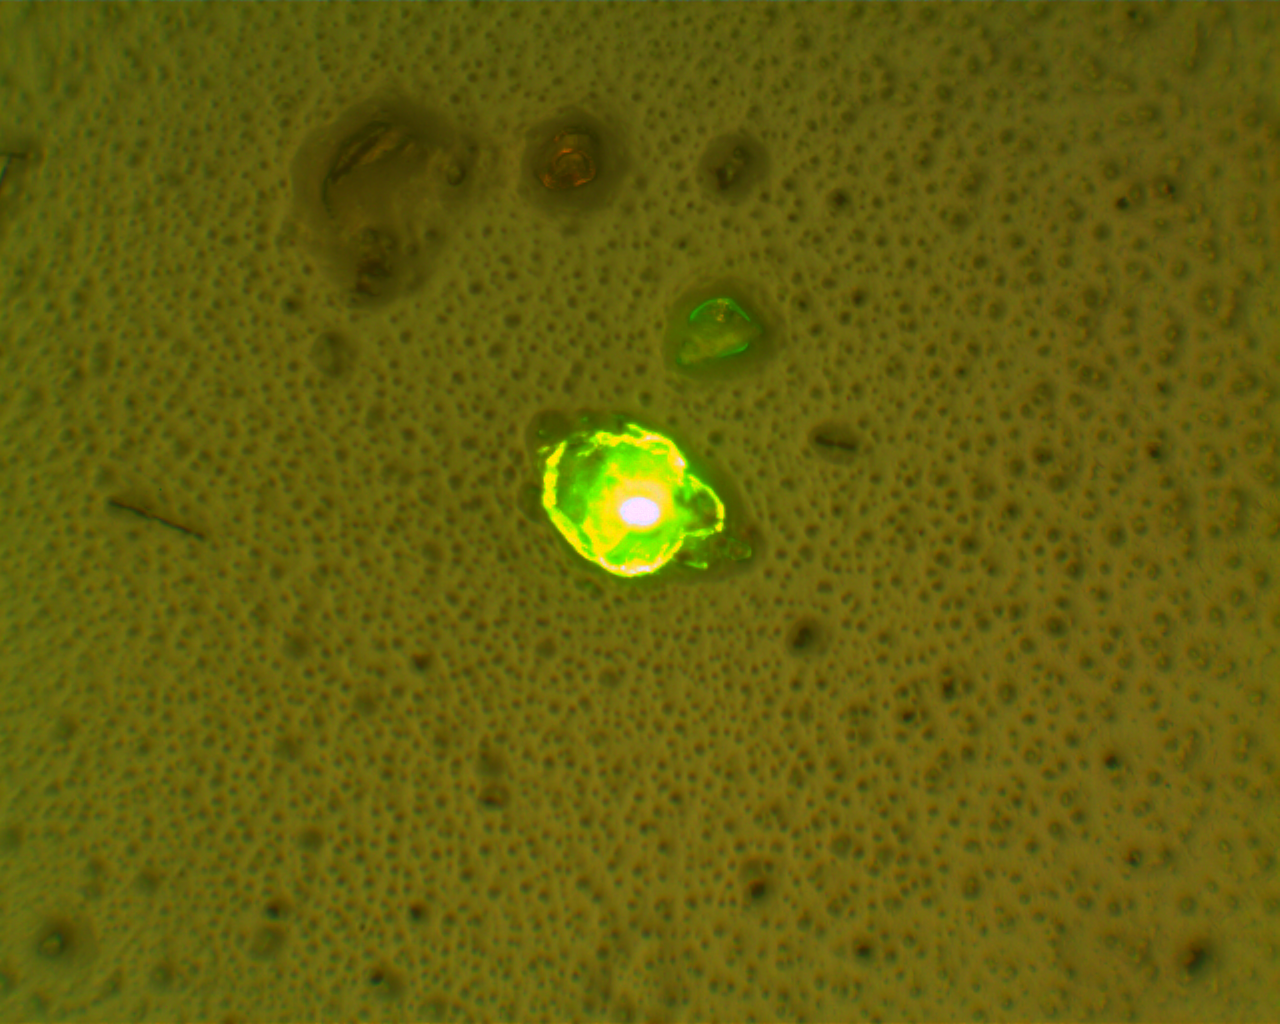
\includegraphics[width=4cm]{./img/qd-laser-illum.png}
    \caption{PL emission spectrum of a cluster of CdSe quantum dots on ?? substrate, excited at 405 nm. Unlike measurements on ADT, these measurements were taken in a region of interest which is sparsely populated with quantum dots, with one target grouping illuminated by the laser.}
    \label{fig:pl-adt-qd}
\end{figure}

\section{\ce{MoS2}}

[\textbf{Coming soon.}]